\section{Detalles de los modelos}
\label{ap:modelos}



\subsection*{Hiperparámetros}

Los espacios de búsqueda están en la tabla~\ref{tab:espacios}. La tabla~\ref{tab:hiper} muestra los valores elegidos para cada modelo. Las búsquedas de regresión y de clasificación usaron la misma semilla y, por tanto, la misma secuencia de configuraciones; en Random Forest, la configuración 20 fue la mejor en ambas tareas, por lo que sus hiperparámetros coinciden. Se verificó en los archivos de la búsqueda que no se trata de un error de transcripción. La figura~\ref{fig:busqueda} muestra el mejor resultado de validación según el número de configuraciones evaluadas. Todas las búsquedas se detuvieron con las 40 configuraciones iniciales, salvo la de XGBoost en regresión: su mejor configuración fue la 39, de modo que la mejora en las últimas diez superó la tolerancia y la búsqueda se amplió a 60 configuraciones, sin nuevas mejoras.

\begin{figure}[htbp]\centering
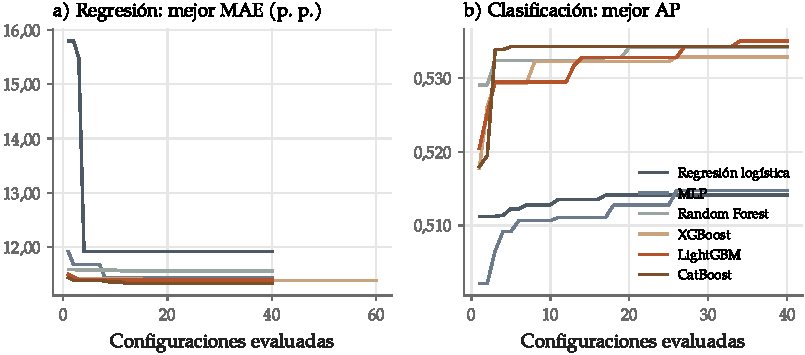
\includegraphics[width=.8\textwidth]{fig_busqueda}
\caption{Convergencia de la búsqueda aleatoria: mejor MAE promedio de validación (a) y mejor AP de validación (b) según el número de configuraciones evaluadas.}\label{fig:busqueda}
\end{figure}
\FloatBarrier

\footnotesize
\begin{longtable}{llrp{7.4cm}}
\caption{Hiperparámetros elegidos por búsqueda aleatoria (número de configuraciones evaluadas en la tercera columna). Las dos búsquedas de cada modelo usaron la misma semilla y, por tanto, la misma secuencia de configuraciones; en Random Forest, la misma configuración resultó la mejor en ambas tareas, por lo que sus valores coinciden.}\label{tab:hiper}\\
\toprule Tarea & Modelo & $N$ & Valores elegidos\\ \midrule\endfirsthead
\toprule Tarea & Modelo & $N$ & Valores elegidos\\ \midrule\endhead
\bottomrule\endfoot
Reg. & Regresión cuantílica & 40 & $\alpha$ $3{,}4\cdot10^{-7}$; penal. L1 \\
Reg. & MLP & 40 & $\alpha$ 0{,}0067; capas (128, 64); tasa 0{,}0019 \\
Reg. & Random Forest & 40 & hoja mín. 21; frac. var. 0{,}405; prof. 19 \\
Reg. & XGBoost & 60 & frac. col. 0{,}451; tasa 0{,}022; peso mín. 7{,}370; árboles 424; prof. 7; submuestra 0{,}751 \\
Reg. & LightGBM & 40 & frac. col. 0{,}636; hojas 33; $\lambda$ 0{,}0019; tasa 0{,}023; obs. hoja 135; árboles 581; submuestra 0{,}948 \\
Reg. & CatBoost & 40 & $\lambda$ 2{,}288; tasa 0{,}044; árboles 307; prof. 7 \\
\midrule
Clas. & Regresión logística & 40 & $C$ 0{,}0030; penal. L1 \\
Clas. & MLP & 40 & $\alpha$ $1{,}9\cdot10^{-5}$; capas (64); tasa $2{,}0\cdot10^{-4}$ \\
Clas. & Random Forest & 40 & hoja mín. 21; frac. var. 0{,}405; prof. 19 \\
Clas. & XGBoost & 40 & frac. col. 0{,}573; tasa 0{,}040; peso mín. 21{,}485; árboles 190; prof. 6; submuestra 0{,}637 \\
Clas. & LightGBM & 40 & frac. col. 0{,}722; hojas 89; $\lambda$ 9{,}149; tasa 0{,}029; obs. hoja 83; árboles 166; submuestra 0{,}705 \\
Clas. & CatBoost & 40 & $\lambda$ 4{,}448; tasa 0{,}039; árboles 447; prof. 4 \\
Cuant. & LightGBM & 40 & frac. col. 0{,}808; hojas 12; $\lambda$ 8{,}209; tasa 0{,}025; obs. hoja 106; árboles 611; submuestra 0{,}765 \\
\end{longtable}
\normalsize


\clearpage
\subsection*{Verificación de las implementaciones propias}

La regresión cuantílica por descenso de gradiente se comparó con la solución exacta en una submuestra; la red neuronal con pérdida absoluta, comparando su gradiente con diferencias finitas y comprobando en datos simulados que estima la mediana y no la media, y el Random Forest de LightGBM, con el de scikit-learn con los mismos hiperparámetros. Las tres coinciden con su referencia (tabla~\ref{tab:verificacion}). En la regresión cuantílica, la correlación entre los coeficientes (0,77) es menor que entre las predicciones (0,998), porque varias variables están muy correlacionadas entre sí y distintas combinaciones de coeficientes dan casi el mismo ajuste. El bosque de LightGBM tiene un error 0,19 puntos mayor que el de scikit-learn en la submuestra, con predicciones muy correlacionadas.

\begin{table}[htbp]\centering\footnotesize
\caption{Verificación de las implementaciones no estándar (submuestras de 6\,000 y 3\,000 filas de entrenamiento, 4\,000 de validación; simulación con ruido exponencial centrado en la mediana)}\label{tab:verificacion}
\begin{adjustbox}{max width=\textwidth}\begin{tabular}{llr}\toprule
Implementación & Comprobación & Resultado\\ \midrule
Regresión cuantílica & MAE (p.\,p.) solución exacta / descenso de gradiente & 11{,}58 / 11{,}59 \\
 & Correlación de predicciones / de coeficientes & 0{,}9979 / 0{,}769 \\
MLP (error absoluto) & Error relativo del gradiente, mediana / máximo & $1{,}8\cdot10^{-9}$ / $8{,}1\cdot10^{-6}$ \\
 & Simulación: distancia a la mediana / a la media (pérdida absoluta) & 0{,}059 / 0{,}334 \\
 & Simulación: distancia a la mediana / a la media (pérdida cuadrática) & 0{,}337 / 0{,}045 \\
Random Forest & MAE (p.\,p.) LightGBM / scikit-learn / paseo aleatorio & 11{,}81 / 11{,}62 / 13{,}43 \\
 & Correlación de predicciones & 0{,}954 \\
\bottomrule\end{tabular}\end{adjustbox}\end{table}



